\section{Monitors module}


The most important step in order to adapt, is to acquire insight on the current behavior of the application EFP of interest, which defines the performance of the application.
For example, the application developer might be interested on the execution time of the kernel or in the accuracy of the result.
While the first metric might be applied to every class of applications, the accuracy of the result is meaningful only in the context of an application.
For example, a video encoder might use the Peak to Signal Noise Ration (PSNR) as accuracy metric, while a scientific application might be more interested on the difference between the actual result and the ground truth value.

\begin{figure}
	\centering
	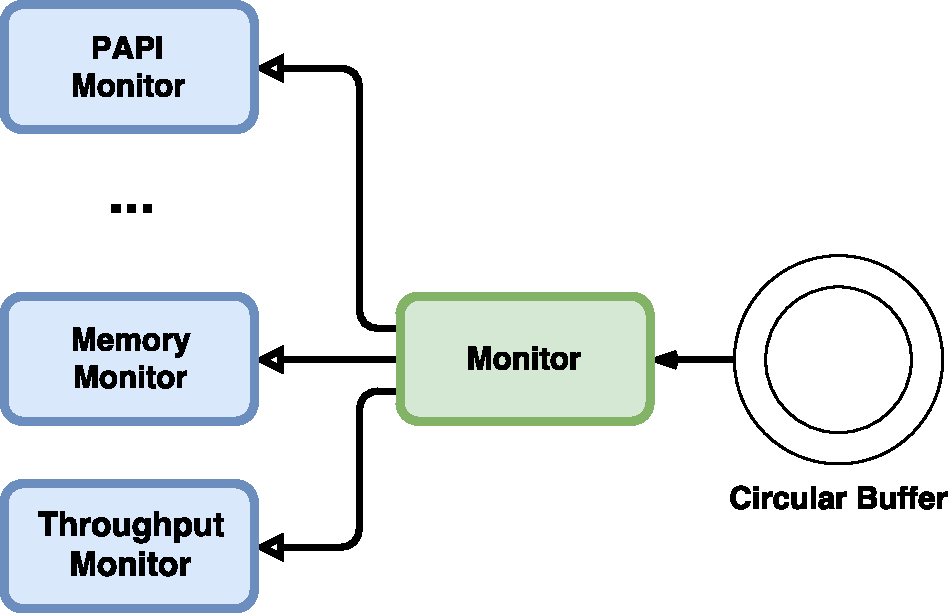
\includegraphics[scale=0.5]{monitor_modules}
	\caption{Overview of the monitors module. }
	\label{fig:monitor_module}
\end{figure}

For this reason the monitors module must be flexible enough to let the user to define custom monitor to observe application-specific metrics.
\prettyref{fig:monitor_module} shows the overview of the structure of the monitors module.
A base class (\textit{Monitor}) implements a circular buffer which store the last \textit{n} (user defined) observations and provides to the user the possibility to extract statistical properties over observed data.
Moreover, this class implements all the methods required to interact with all the other framework elements.
It is possible to specify the type of the elements stored in the circular buffer and the precision used to compute the statistical properties (by default it uses at least 32bit float).
Each time a statistical properties is computed, the monitor uses a cache-like mechanism to avoid to recompute the property.


The actual monitor must extend the latter class, with the functionality that actually gather the target metric and push the value in the circular buffer (using the \textit{push}) method.
mARGOt ships with the following suite of monitors:

\begin{itemize}
	\item Energy monitor (uses the RAPL environment)
	\item Frequency monitor (uses the CPUfreq environment)
	\item Memory monitor
	\item Odroid power monitor
	\item Odroid energy monitor
	\item PAPI monitor (uses the PAPI environment)
	\item Process and system CPU usage
	\item Temperature monitor (uses the Sensors environment)
	\item Throughput monitor
	\item Time monitor
\end{itemize}


\begin{figure}[!t]
	\centering
	\lstset{language=MyCPP}
	\begin{lstlisting}
	// monitor definitions
	margot::Monitor<float> my_float_monitor(3);
	margot::Monitor<int, double> my_int_monitor;
	margot::Monitor<double>  my_double_monitor;
	margot::TimeMonitor timer;
	
	// how to observe a metric
	timer.start();
	timer.stop()
	my_float_monitor.push(3.2f);
	
	// how to extract statistical properties
	const auto avg_time = timer.average();
	const auto avg_float = my_float_monitor.average();
	\end{lstlisting}
	\caption{Example of C++ code to define and use monitors.}
	\label{fig:monitor_examples}
\end{figure}

\prettyref{fig:monitor_examples} shows some examples on how it is possible to define and use monitors.
In particular, line 1 defines a basic monitor which stores float and has a circular buffer of three elements.
Line 2 defines a monitor of integer, however it specify that the statistical properties such as average and standard deviation should be performed using 64bit of precision. 
Moreover, the default constructor set the circular buffer size to just one element.
Line 3 defines a monitor of doubles.
Since the default type used to compute statistical properties is a float, mARGOt automatically promote the latter to double, to prevent precision loss.
Line 4 defines a time monitor, which is a specialization of the generic monitor, suitable to record the elapsed time from a start and stop method (lines 8,9).
In general each specialized monitor provides its own method to observe the target metric.
For a full description of each monitor, refer to the doxygen documentation.
To ``observe'' a value using a custom monitor (line 10), it is required to use the \textit{push} method.
Regardless of the monitor type, to extract statistical properties (lines 13-14), it is enough to use the dedicated method.
In particular, it is possible to extract the following statistical properties (defined in the enum \textit{DataFunctions}):

\begin{itemize}
	\item Average
	\item Standard deviation
	\item Maximum element observed
	\item Minimum element observed
\end{itemize}


\subsection{Application Goals}

\begin{figure}[!t]
	\centering
	\lstset{language=MyCPP}
	\begin{lstlisting}
	margot::TimeMonitor timer(margot::TimeUnit::MILLISECONDS);
	margot::Goal<int, margot::ComparisonFunctions::LESS> my_goal(2);
	
	timer.start();
	
	// application kernel
	
	timer.stop();
	
	if (my_goal.check<float,float,margot::DataFunctions::AVERAGE>(timer))
	{
		std::cout << "We are fast" << std::endl;
	}
	else
	{
		std::cout << "We should improve" << std::endl;
	}
	\end{lstlisting}
	\caption{Example of C++ code to check if the elapsed time to execute the application kernel is below $2ms$.}
	\label{fig:goal_examples}
\end{figure}

Since the application developer might have requirements on the lower bound or upper bound on a metric of interest.
mARGOt uses the class \textit{Goal} to represents this concept.
In particular, it is possible to test if a statistical properties of the monitor achieve the goal or to compute its absolute o relative error.
In the current implementation, a support four standard comparison functions (greater than, grater or equal than, less than and less or equal than), defined in the enum \textit{ComparisonFunctions}.

\prettyref{fig:goal_examples} shows an example on how it is possible to use the goals and monitors, to check if the application kernel execution time is below $2ms$.
In particular, line 1 defines a time monitor with a resolution of milliseconds.
Line 2 defines a goal with value $2$ and comparison function ``less than'', the numerical value of the goal might be changed dynamically.
After that we have instrumented the kernel of the application (lines 4-8), we check if the execution time was below $2ms$ (line 10), and we print an output message accordingly (lines 10-17). 

 
 

 